%% SPDX-License-Identifier: MIT
%% SPDX-FileCopyrightText: 2012-2016, Sven Eckelmann <sven@narfation.org>

\documentclass[a4paper,10pt,twoside]{article}
\usepackage{tikz}
\usetikzlibrary{shapes}
\usetikzlibrary{arrows}
\usepackage{pslatex}
\usepackage{amssymb}
\usepackage{textcomp}
\usepackage{parskip}
\usepackage{graphicx}
\usepackage{txfonts}
\usepackage{listings}
\usepackage[T1]{fontenc}

\usepackage[ps2pdf]{thumbpdf}
\usepackage[pdftex,backref]{hyperref}
\hypersetup{%
   pdfauthor={Sven Eckelmann}
   pdftitle={Nonrecursive Left-Leaning Red-Black 2-3 Tree}
   bookmarksnumbered=true,
   pdfstartview={FitH},
   colorlinks=true,
   linkcolor=black,
   plainpages = false
}


\tikzset{
	treenode/.style = {
		align=center,
		inner sep=0pt,
		text centered,
		font=\sffamily,
		anchor=north
	},
	node_b/.style = {
		treenode,
		circle,
		white,
		font=\sffamily\bfseries,
		draw=black,
		fill=black,
		text width=1.5em
	},
	node_r/.style = {
		treenode,
		circle,
		red,
		draw=red,
		text width=1.5em,
		very thick
	},
	node_rb/.style = {
		treenode,
		circle,
		black,
		draw=black,
		fill=white,
		text width=1.5em,
		thin
	},
	node_nil/.style = {
		treenode,
		rectangle,
		draw=black,
		draw=black,
		fill=black,
		minimum width=0.5em,
		minimum height=0.5em
	},
	node_tree/.style = {
		treenode,
		isosceles triangle, isosceles triangle stretches,
		shape border rotate=90,
		isosceles triangle apex angle=50,
		inner sep=1,
		draw=black,
		anchor=north,
		text width=1.5em,
		minimum height=3.0em
	},
	node_tree_low/.style = {
		node_tree,
		dashed
	},
	node_tree_high1/.style = {
		node_tree,
		minimum height=4.85em
	},
}

\date{}
\author{Sven Eckelmann}
\title{Nonrecursive Left-Leaning Red-Black 2-3 Tree}

\begin{document}

\maketitle
\pagenumbering{roman}
\pdfbookmark[1]{\contentsname}{toc}
\tableofcontents
\cleardoublepage
\pagenumbering{arabic}

\section{Insert}

New nodes are always inserted as red leaf. Such an insert could violate
the basic properties of the LLRB 2-3-node tree. A rebalance has to be initiated
after the insert to fix them. The rebalance is started at the new leaf node
and continues upwards the tree until the root node is reached.

The binary search tree insert, which guarantees the correct order, has to be
implemented outside the red black tree functionality. The insert rebalancing
will take care of not violating BST properties while restoring the (LL)RB
properties of the tree.

\begin{lstlisting}[language=C]
void rbitem_insert(struct rb_root *root,
                   struct rbitem *new_entry)
{
    struct rb_node *parent = NULL;
    struct rb_node **cur_nodep = &root->node;
    struct rbitem *cur_entry;

    /* search correct leaf position in tree */
    while (*cur_nodep) {
        cur_entry = rb_entry(*cur_nodep,
                             struct rbitem, rb);

        parent = *cur_nodep;
        if (cmp(&new_entry->i, &cur_entry->i) <= 0)
            cur_nodep = &(*cur_nodep)->left;
        else
            cur_nodep = &(*cur_nodep)->right;
    }

    /* insert as red leaf + rebalance */
    rb_insert(&new_entry->rb, parent,
              cur_nodep, &queue->root);
}
\end{lstlisting}

\newpage
\section{Insert Rebalance}

%%%%%%%%%%%%%%%%%%%%%%%%%%%%%%%%%%%%%%%%%%%%%%%%%%%%%%%%%%%%%%%%%%%%%%%%%%%%%%%%
% rb_insert_color 3-node rotate to left
%%%%%%%%%%%%%%%%%%%%%%%%%%%%%%%%%%%%%%%%%%%%%%%%%%%%%%%%%%%%%%%%%%%%%%%%%%%%%%%%
\subsection{Right-Leaning 3-node}

\subsubsection{Prerequisites}

\begin{center}
\begin{tabular}{|r||l|l|}
\hline
node		&	black height	&	comment	\\
\hline
\hline
$n$		&	-	&		\\\hline
$y$		&	$h$	&	is red and a right child	\\\hline
$\alpha$	&	$h$	&	root of $\alpha$ must be black or NULL	\\\hline
$\beta$		&	$h$	&		\\\hline
$\gamma$	&	$h$	&		\\\hline
\end{tabular}
\end{center}

The right child of the current node is red. This is a violation of the
left-leaning property for 3-nodes.

\begin{center}
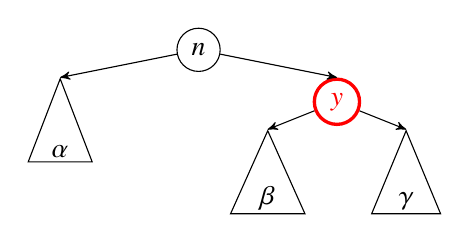
\begin{tikzpicture}[->,>=stealth',level/.style={sibling distance = 10em/#1, level distance = 1em}, child anchor=north]
\node [node_rb] {$n$}
child {
	node [node_tree] {$\alpha$}
}
child {
	node [node_r] {$y$}
	child {
		node [node_tree] {$\beta$}
	}
	child {
		node [node_tree] {$\gamma$}
	}
}
;
\end{tikzpicture}
\end{center}

\subsubsection{Transformation}

\begin{enumerate}
\item A rotation of $n$ to the left resolves this problem without modifying the
black height of the subtree. Two consecutive left red nodes cannot happen
because one prerequisite for this transformation is that root of $\alpha$ must
be black or NULL.

\begin{center}
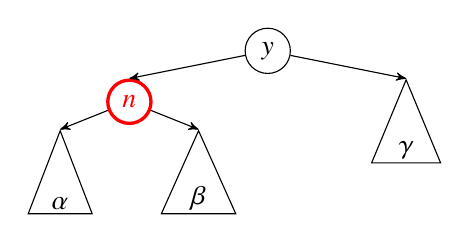
\begin{tikzpicture}[->,>=stealth',level/.style={sibling distance = 10em/#1, level distance = 1em}, child anchor=north]
\node [node_rb] {$y$}
child {
	node [node_r] {$n$}
	child {
		node [node_tree] {$\alpha$}
	}
	child {
		node [node_tree] {$\beta$}
	}
}
child {
	node [node_tree] {$\gamma$}
}
;
\end{tikzpicture}
\end{center}


\item The transformation can be stopped when $y$ is black. A red $y$ can be part
of a property violation and the checks have to be continued at the parent of
$y$.

\end{enumerate}


%%%%%%%%%%%%%%%%%%%%%%%%%%%%%%%%%%%%%%%%%%%%%%%%%%%%%%%%%%%%%%%%%%%%%%%%%%%%%%%%
% rb_insert_color two consecutive left red nodes rotate to right
%%%%%%%%%%%%%%%%%%%%%%%%%%%%%%%%%%%%%%%%%%%%%%%%%%%%%%%%%%%%%%%%%%%%%%%%%%%%%%%%
\newpage
\subsection{Two consecutive left red nodes}

\subsubsection{Prerequisites}

\begin{center}
\begin{tabular}{|r||l|l|}
\hline
node		&	black height	&	comment	\\
\hline
\hline
$n$		&	$h+1$	&	is black	\\\hline
$x$		&	$h$	&	is red	\\\hline
$y$		&	$h$	&	is red	\\\hline
$\alpha$	&	$h$	&		\\\hline
$\beta$		&	$h$	&		\\\hline
$\gamma$	&	$h$	&		\\\hline
$\delta$	&	$h$	&		\\\hline
\end{tabular}
\end{center}

The left child and left-left grandchild of $n$ are red. This violates the
maximum height property of the left subtree which must have an upper bound of
twice the black height + 1.

\begin{center}
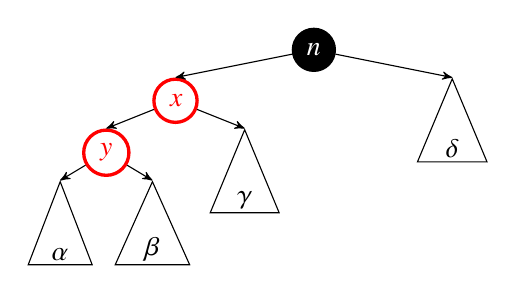
\begin{tikzpicture}[->,>=stealth',level/.style={sibling distance = 10em/#1, level distance = 1em}, child anchor=north]
\node [node_b] {$n$}
child {
	node [node_r] {$x$}
	child {
		node [node_r] {$y$}
		child {
			node [node_tree] {$\alpha$}
		}
		child {
			node [node_tree] {$\beta$}
		}
	}
	child {
			node [node_tree] {$\gamma$}
	}
}
child {
	node [node_tree] {$\delta$}
}
;
\end{tikzpicture}
\end{center}

\subsubsection{Transformation}

\begin{enumerate}
\item A rotation of $n$ to the right resolves this problem without modifying the
black height of the subtree.

\begin{center}
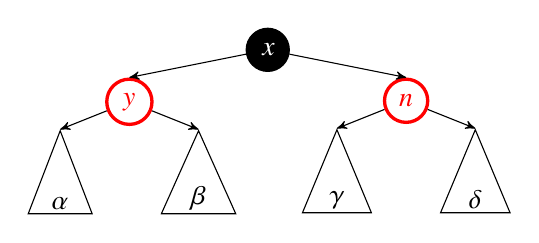
\begin{tikzpicture}[->,>=stealth',level/.style={sibling distance = 10em/#1, level distance = 1em}, child anchor=north]
\node [node_b] {$x$}
child {
	node [node_r] {$y$}
	child {
		node [node_tree] {$\alpha$}
	}
	child {
		node [node_tree] {$\beta$}
	}
}
child {
	node [node_r] {$n$}
	child {
		node [node_tree] {$\gamma$}
	}
	child {
		node [node_tree] {$\delta$}
	}
}
;
\end{tikzpicture}
\end{center}


\item The previous transformation creates a 4-node. This is a violation for a
2-3 node LLRB tree. This can be solved by the transformation described in
\nameref{insert_both_children_red}.

\end{enumerate}


%%%%%%%%%%%%%%%%%%%%%%%%%%%%%%%%%%%%%%%%%%%%%%%%%%%%%%%%%%%%%%%%%%%%%%%%%%%%%%%%
% rb_insert_color both children red recolor
%%%%%%%%%%%%%%%%%%%%%%%%%%%%%%%%%%%%%%%%%%%%%%%%%%%%%%%%%%%%%%%%%%%%%%%%%%%%%%%%
\newpage
\subsection{Both children red}
\label{insert_both_children_red}

\subsubsection{Prerequisites}

\begin{center}
\begin{tabular}{|r||l|l|}
\hline
node		&	black height	&	comment	\\
\hline
\hline
$n$		&	$h+1$	&	is black	\\\hline
$x$		&	$h$	&	is red	\\\hline
$y$		&	$h$	&	is red	\\\hline
$\alpha$	&	$h$	&		\\\hline
$\beta$		&	$h$	&		\\\hline
$\gamma$	&	$h$	&		\\\hline
$\delta$	&	$h$	&		\\\hline
\end{tabular}
\end{center}

A 4-node is not allowed in the 2-3 node variant of the LLRB tree.

\begin{center}
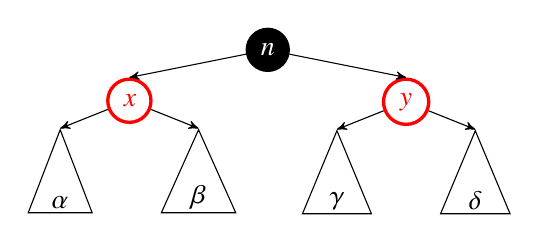
\begin{tikzpicture}[->,>=stealth',level/.style={sibling distance = 10em/#1, level distance = 1em}, child anchor=north]
\node [node_b] {$n$}
child {
	node [node_r] {$x$}
	child {
		node [node_tree] {$\alpha$}
	}
	child {
		node [node_tree] {$\beta$}
	}
}
child {
	node [node_r] {$y$}
	child {
		node [node_tree] {$\gamma$}
	}
	child {
		node [node_tree] {$\delta$}
	}
}
;
\end{tikzpicture}
\end{center}

\subsubsection{Transformation}

\begin{enumerate}
\item The subtree already has the right black height. All modifications
therefore have to keep the black height the same. The flipping of colors for
$n$, $x$ and $y$ will split the 4-node while keeping the black height.

\begin{center}
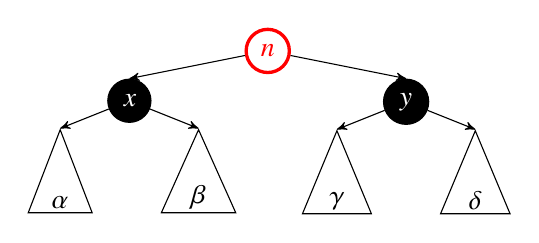
\begin{tikzpicture}[->,>=stealth',level/.style={sibling distance = 10em/#1, level distance = 1em}, child anchor=north]
\node [node_r] {$n$}
child {
	node [node_b] {$x$}
	child {
		node [node_tree] {$\alpha$}
	}
	child {
		node [node_tree] {$\beta$}
	}
}
child {
	node [node_b] {$y$}
	child {
		node [node_tree] {$\gamma$}
	}
	child {
		node [node_tree] {$\delta$}
	}
}
;
\end{tikzpicture}
\end{center}


\item The red node $n$ can be part
of a property violation and the checks have to be continued at the parent of
$n$.

\end{enumerate}


%%%%%%%%%%%%%%%%%%%%%%%%%%%%%%%%%%%%%%%%%%%%%%%%%%%%%%%%%%%%%%%%%%%%%%%%%%%%%%%%
% rb_insert_color root node is red
%%%%%%%%%%%%%%%%%%%%%%%%%%%%%%%%%%%%%%%%%%%%%%%%%%%%%%%%%%%%%%%%%%%%%%%%%%%%%%%%
\newpage
\subsection{Root is red}

\subsubsection{Prerequisites}

\begin{center}
\begin{tabular}{|r||l|l|}
\hline
node		&	black height	&	comment	\\
\hline
\hline
$n$		&	$h$	&	is red and the root of the tree	\\\hline
$\alpha$	&	$h$	&		\\\hline
$\beta$		&	$h$	&		\\\hline
\end{tabular}
\end{center}

A root of a tree always has to be black.

\begin{center}
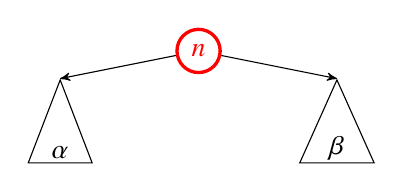
\begin{tikzpicture}[->,>=stealth',level/.style={sibling distance = 10em/#1, level distance = 1em}, child anchor=north]
\node [node_r] {$n$}
child {
	node [node_tree] {$\alpha$}
}
child {
	node [node_tree] {$\beta$}
}
;
\end{tikzpicture}
\end{center}

\subsubsection{Transformation}

\begin{enumerate}
\item Changing the color of $n$ increases the black height of the tree. But
no imbalance can be introduced because $\alpha$ and $\beta$ are already balanced
and $n$ has no parent which could get imbalanced.

\begin{center}
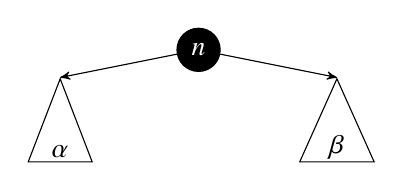
\begin{tikzpicture}[->,>=stealth',level/.style={sibling distance = 10em/#1, level distance = 1em}, child anchor=north]
\node [node_b] {$n$}
child {
	node [node_tree] {$\alpha$}
}
child {
	node [node_tree] {$\beta$}
}
;
\end{tikzpicture}
\end{center}


\item Rebalance can always always stop after $n$ is marked as black.

\end{enumerate}


\newpage
\section{Delete}

The deletion of nodes can only happen at a leaf node or at a internal node with
only one (left) child. If an internal node with two children must be deleted
then it has to be be replaced by a leaf node. This replacement can either be the
rightmost child in the left subtree or the leftmost child in the right subtree.

A replacement node will be inserted in the place of the internal node with two
children. The replacement node will receive the color
of the internal node. The actual removal of a node happened further down the
tree. Thus all further rebalancing operations have to start at the original
position of the replacement node.

A removed red node can never cause a subtree with imbalanced black height. Such
a removal therefore never has to start the rebalancing process. The delete
rebalancing will take care of fixing a imbalance caused by a removal of a black
node.

All this is implemented in \verb|rb_erase|.

%%%%%%%%%%%%%%%%%%%%%%%%%%%%%%%%%%%%%%%%%%%%%%%%%%%%%%%%%%%%%%%%%%%%%%%%%%%%%%%%
% delete leaf
%%%%%%%%%%%%%%%%%%%%%%%%%%%%%%%%%%%%%%%%%%%%%%%%%%%%%%%%%%%%%%%%%%%%%%%%%%%%%%%%
\subsection{Delete leaf node}
\label{delete_leaf_node}

\subsubsection{Prerequisites}

\begin{center}
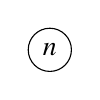
\begin{tikzpicture}[->,>=stealth',level/.style={sibling distance = 10em/#1, level distance = 1em}, child anchor=north]
\node [node_rb] {$n$}
;
\end{tikzpicture}
\end{center}

\subsubsection{Transformation}

\begin{enumerate}
\item The leave node $n$ can simply be removed. When $n$ was black then the
rebalance to fix the black height imbalance has to be started at its parent.

\begin{center}
\begin{tikzpicture}[->,>=stealth',level/.style={sibling distance = 10em/#1, level distance = 1em}, child anchor=north]
;
\end{tikzpicture}
\end{center}


\end{enumerate}

%%%%%%%%%%%%%%%%%%%%%%%%%%%%%%%%%%%%%%%%%%%%%%%%%%%%%%%%%%%%%%%%%%%%%%%%%%%%%%%%
% delete internal node with onlu left child
%%%%%%%%%%%%%%%%%%%%%%%%%%%%%%%%%%%%%%%%%%%%%%%%%%%%%%%%%%%%%%%%%%%%%%%%%%%%%%%%
\subsection{Delete internal node with only left child}

\subsubsection{Prerequisites}

\begin{center}
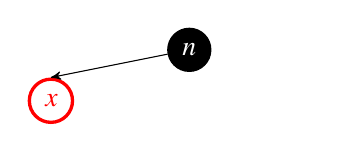
\begin{tikzpicture}[->,>=stealth',level/.style={sibling distance = 10em/#1, level distance = 1em}, child anchor=north]
\node [node_b] {$n$}
child {
	node [node_r] {$x$}
}
child {
	[white]
}
;
\end{tikzpicture}
\end{center}

\subsubsection{Transformation}

\begin{enumerate}
\item The node $n$ can simply be removed. $x$ moves up one level and replaces
$n$.

\begin{center}

\begin{tikzpicture}[->,>=stealth',level/.style={sibling distance = 10em/#1, level distance = 1em}, child anchor=north]
\node [node_r] {$x$}
;
\end{tikzpicture}
\end{center}


\item The deletion of the black $n$ caused an black height imbalance. This can
simply be solved by recoloring the red $x$ as to black.

\begin{center}

\begin{tikzpicture}[->,>=stealth',level/.style={sibling distance = 10em/#1, level distance = 1em}, child anchor=north]
\node [node_b] {$x$}
;
\end{tikzpicture}
\end{center}

\end{enumerate}



%%%%%%%%%%%%%%%%%%%%%%%%%%%%%%%%%%%%%%%%%%%%%%%%%%%%%%%%%%%%%%%%%%%%%%%%%%%%%%%%
% delete internal node with two childred
%%%%%%%%%%%%%%%%%%%%%%%%%%%%%%%%%%%%%%%%%%%%%%%%%%%%%%%%%%%%%%%%%%%%%%%%%%%%%%%%
\subsection{Delete internal node with two children}

\subsubsection{Prerequisites}

\begin{center}
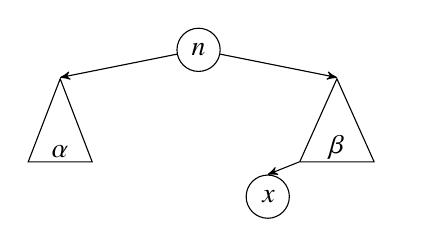
\begin{tikzpicture}[->,>=stealth',level/.style={sibling distance = 10em/#1, level distance = 1em}, child anchor=north]
\node [node_rb] {$n$}
child {
	node [node_tree] {$\alpha$}
}
child {
	node [node_tree] {$\beta$}
	child {
		node [node_rb] {$x$}
	}
	child {
		[white]
	}
}
;
\end{tikzpicture}
\end{center}

\subsubsection{Transformation}

\begin{enumerate}
\item The leftmost node ($x$) in the right subtree of $n$ has to be found. $x$
is used to replace $n$ in the tree. $x$ becomes red when $n$ was red and black
when $n$ was black.

\begin{center}
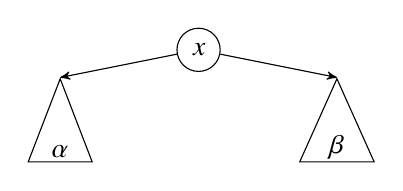
\begin{tikzpicture}[->,>=stealth',level/.style={sibling distance = 10em/#1, level distance = 1em}, child anchor=north]
\node [node_rb] {$x$}
child {
	node [node_tree] {$\alpha$}
}
child {
	node [node_tree] {$\beta$}
}
;
\end{tikzpicture}
\end{center}


\item The removal of $x$ worked as explained in \nameref{delete_leaf_node}. The
delete rebalancing therefore has to be started at the previous parent of $x$.

\end{enumerate}


\newpage
\section{Delete Rebalance}

%%%%%%%%%%%%%%%%%%%%%%%%%%%%%%%%%%%%%%%%%%%%%%%%%%%%%%%%%%%%%%%%%%%%%%%%%%%%%%%%
% rb_erase_left_restructure
%%%%%%%%%%%%%%%%%%%%%%%%%%%%%%%%%%%%%%%%%%%%%%%%%%%%%%%%%%%%%%%%%%%%%%%%%%%%%%%%
\subsection{Low Left Subtree, Restructure}

\subsubsection{Prerequisites}

\begin{center}
\begin{tabular}{|r||l|l|}
\hline
node		&	black height	&	comment	\\
\hline
\hline
$p$		&	imbalanced	&		\\\hline
$x$		&	$h$	&	is red	\\\hline
$s$		&	$h+1$	&	black sibling of $\epsilon$ root	\\\hline
$\epsilon$	&	$h$	&	black node was removed from subtree, left child of $p$	\\\hline
$\alpha$	&	$h$	&		\\\hline
$\beta$		&	$h$	&		\\\hline
$\gamma$	&	$h$	&		\\\hline
\end{tabular}
\end{center}

\begin{center}
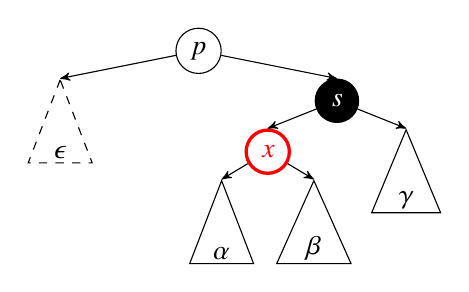
\begin{tikzpicture}[->,>=stealth',level/.style={sibling distance = 10em/#1, level distance = 1em}, child anchor=north]
\node [node_rb] {$p$}
child {
	node [node_tree_low] {$\epsilon$}
}
child {
	node [node_b] {$s$}
	child {
		node [node_r] {$x$}
		child {
			node [node_tree] {$\alpha$}
		}
		child {
			node [node_tree] {$\beta$}
		}
	}
	child {
		node [node_tree] {$\gamma$}
	}
}
;
\end{tikzpicture}
\end{center}

\subsubsection{Transformation}

\begin{enumerate}
\item The black node from the right subtree has to be transferred to the left
to increase its height. But at first the right subtree has to be prepared
to avoid a reduction of its black height. This is done by rotating $s$ to the
right and thereby creating a right leaning 3-node.

\begin{center}
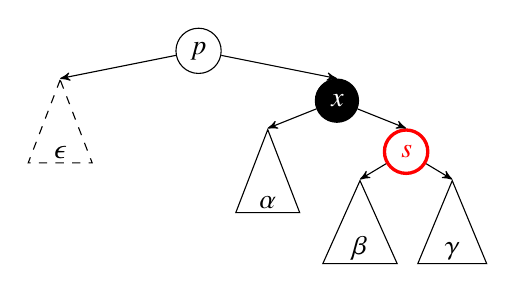
\begin{tikzpicture}[->,>=stealth',level/.style={sibling distance = 10em/#1, level distance = 1em}, child anchor=north]
\node [node_rb] {$p$}
child {
	node [node_tree_low] {$\epsilon$}
}
child {
	node [node_b] {$x$}
	child {
		node [node_tree] {$\alpha$}
	}
	child {
		node [node_r] {$s$}
		child {
			node [node_tree] {$\beta$}
		}
		child {
			node [node_tree] {$\gamma$}
		}
	}
}
;
\end{tikzpicture}
\end{center}


\item $p$ can now be rotated to the left to fix the black height in the
left subtree.

\begin{center}
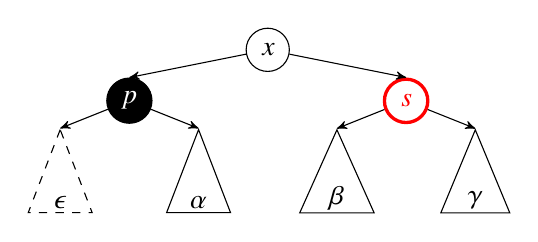
\begin{tikzpicture}[->,>=stealth',level/.style={sibling distance = 10em/#1, level distance = 1em}, child anchor=north]
\node [node_rb] {$x$}
child {
	node [node_b] {$p$}
	child {
		node [node_tree_low] {$\epsilon$}
	}
	child {
		node [node_tree] {$\alpha$}
	}
}
child {
	node [node_r] {$s$}
	child {
		node [node_tree] {$\beta$}
	}
	child {
		node [node_tree] {$\gamma$}
	}
}
;
\end{tikzpicture}
\end{center}


\item The right subtree now has a too low black height compared to the left
tree. But the red $s$ can simply be recolored to black to increase the black
height again and to fix the misbalance in the tree. The rebalance process is
finished after that.

\begin{center}
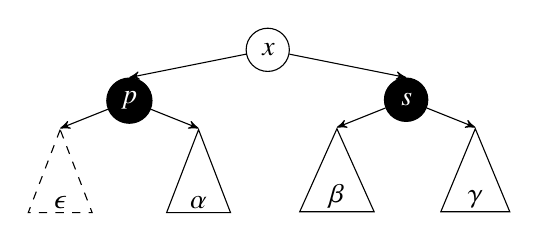
\begin{tikzpicture}[->,>=stealth',level/.style={sibling distance = 10em/#1, level distance = 1em}, child anchor=north]
\node [node_rb] {$x$}
child {
	node [node_b] {$p$}
	child {
		node [node_tree_low] {$\epsilon$}
	}
	child {
		node [node_tree] {$\alpha$}
	}
}
child {
	node [node_b] {$s$}
	child {
		node [node_tree] {$\beta$}
	}
	child {
		node [node_tree] {$\gamma$}
	}
}
;
\end{tikzpicture}
\end{center}


\end{enumerate}


%%%%%%%%%%%%%%%%%%%%%%%%%%%%%%%%%%%%%%%%%%%%%%%%%%%%%%%%%%%%%%%%%%%%%%%%%%%%%%%%
% rb_erase_left_recolor_red
%%%%%%%%%%%%%%%%%%%%%%%%%%%%%%%%%%%%%%%%%%%%%%%%%%%%%%%%%%%%%%%%%%%%%%%%%%%%%%%%
\newpage
\subsection{Low Left Subtree, Recolor under red parent}

\subsubsection{Prerequisites}

\begin{center}
\begin{tabular}{|r||l|l|}
\hline
node		&	black height	&	comment	\\
\hline
\hline
$p$		&	imbalanced	&	is red	\\\hline
$s$		&	$h+1$	&	black sibling of $\epsilon$ root	\\\hline
$\epsilon$	&	$h$	&	black node was removed from subtree, left child of $p$	\\\hline
$\alpha$	&	$h$	&	root of $\alpha$ must be black or NULL	\\\hline
$\beta$		&	$h$	&		\\\hline
\end{tabular}
\end{center}

\begin{center}
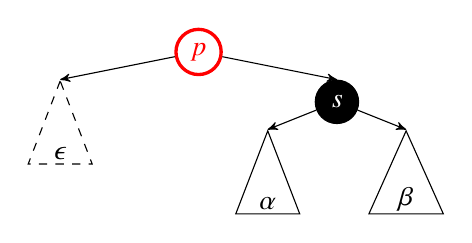
\begin{tikzpicture}[->,>=stealth',level/.style={sibling distance = 10em/#1, level distance = 1em}, child anchor=north]
\node [node_r] {$p$}
child {
	node [node_tree_low] {$\epsilon$}
}
child {
	node [node_b] {$s$}
	child {
		node [node_tree] {$\alpha$}
	}
	child {
		node [node_tree] {$\beta$}
	}
}
;
\end{tikzpicture}
\end{center}

\subsubsection{Transformation}

\begin{enumerate}
\item Switching the colors of $p$ und $s$ fixes the black heights. The black
height of the right subtree is decreased (and therefore equal to the left
subtree) while the black height under $p$ is increased. The imbalance is
solved.

\begin{center}
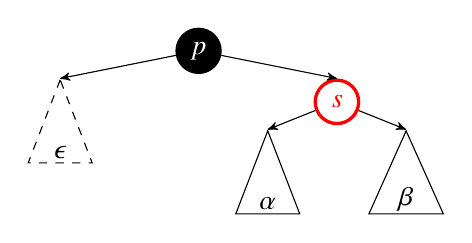
\begin{tikzpicture}[->,>=stealth',level/.style={sibling distance = 10em/#1, level distance = 1em}, child anchor=north]
\node [node_b] {$p$}
child {
	node [node_tree_low] {$\epsilon$}
}
child {
	node [node_r] {$s$}
	child {
		node [node_tree] {$\alpha$}
	}
	child {
		node [node_tree] {$\beta$}
	}
}
;
\end{tikzpicture}
\end{center}


\item This recoloring created a left leaning 3-node. $p$ has to be rotated to
the left to solve this without changing the black height.

\begin{center}
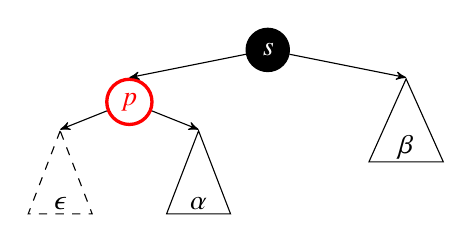
\begin{tikzpicture}[->,>=stealth',level/.style={sibling distance = 10em/#1, level distance = 1em}, child anchor=north]
\node [node_b] {$s$}
child {
	node [node_r] {$p$}
	child {
		node [node_tree_low] {$\epsilon$}
	}
	child {
		node [node_tree] {$\alpha$}
	}
}
child {
	node [node_tree] {$\beta$}
}
;
\end{tikzpicture}
\end{center}


\end{enumerate}


%%%%%%%%%%%%%%%%%%%%%%%%%%%%%%%%%%%%%%%%%%%%%%%%%%%%%%%%%%%%%%%%%%%%%%%%%%%%%%%%
% rb_erase_left_recolor_black
%%%%%%%%%%%%%%%%%%%%%%%%%%%%%%%%%%%%%%%%%%%%%%%%%%%%%%%%%%%%%%%%%%%%%%%%%%%%%%%%
\newpage
\subsection{Low Left Subtree, Recolor under black parent}

\subsubsection{Prerequisites}

\begin{center}
\begin{tabular}{|r||l|l|}
\hline
node		&	black height	&	comment	\\
\hline
\hline
$p$		&	imbalanced	&	is black	\\\hline
$s$		&	$h+1$	&	black sibling of $\epsilon$ root	\\\hline
$\epsilon$	&	$h$	&	black node was removed from subtree, left child of $p$	\\\hline
$\alpha$	&	$h$	&	root of $\alpha$ must be black or NULL	\\\hline
$\beta$		&	$h$	&		\\\hline
\end{tabular}
\end{center}

\begin{center}
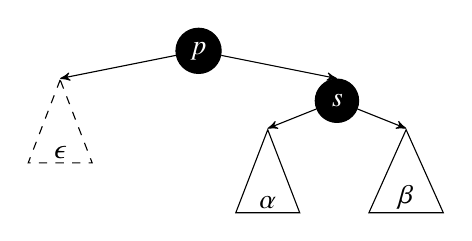
\begin{tikzpicture}[->,>=stealth',level/.style={sibling distance = 10em/#1, level distance = 1em}, child anchor=north]
\node [node_b] {$p$}
child {
	node [node_tree_low] {$\epsilon$}
}
child {
	node [node_b] {$s$}
	child {
		node [node_tree] {$\alpha$}
	}
	child {
		node [node_tree] {$\beta$}
	}
}
;
\end{tikzpicture}
\end{center}

\subsubsection{Transformation}

\begin{enumerate}
\item The imbalance cannot be solved using local operations. Instead the black
height of the right subtree has to be decreased to have the same height as
the left subtree. This is done by recoloring $s$.

\begin{center}
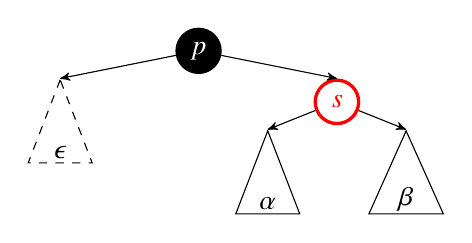
\begin{tikzpicture}[->,>=stealth',level/.style={sibling distance = 10em/#1, level distance = 1em}, child anchor=north]
\node [node_b] {$p$}
child {
	node [node_tree_low] {$\epsilon$}
}
child {
	node [node_r] {$s$}
	child {
		node [node_tree] {$\alpha$}
	}
	child {
		node [node_tree] {$\beta$}
	}
}
;
\end{tikzpicture}
\end{center}


\item The created right-leaning 3-node has to be fixed by rotating $p$ to the
right.

\begin{center}
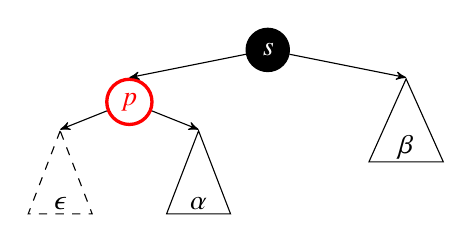
\begin{tikzpicture}[->,>=stealth',level/.style={sibling distance = 10em/#1, level distance = 1em}, child anchor=north]
\node [node_b] {$s$}
child {
	node [node_r] {$p$}
	child {
		node [node_tree_low] {$\epsilon$}
	}
	child {
		node [node_tree] {$\alpha$}
	}
}
child {
	node [node_tree] {$\beta$}
}
;
\end{tikzpicture}
\end{center}


\item The subtree under $s$ has its black height reduced by 1. This problem
has to be propagated further upward the tree to get it solved.

\end{enumerate}


%%%%%%%%%%%%%%%%%%%%%%%%%%%%%%%%%%%%%%%%%%%%%%%%%%%%%%%%%%%%%%%%%%%%%%%%%%%%%%%%
% rb_erase_right_adjust_black
%%%%%%%%%%%%%%%%%%%%%%%%%%%%%%%%%%%%%%%%%%%%%%%%%%%%%%%%%%%%%%%%%%%%%%%%%%%%%%%%
\newpage
\subsection{Low Right Subtree, Adjust with Recolor}

\subsubsection{Prerequisites}

\begin{center}
\begin{tabular}{|r||l|l|}
\hline
node		&	black height	&	comment	\\
\hline
\hline
$p$		&	imbalanced	&	is black	\\\hline
$s$		&	$h+1$	&	red sibling of $\epsilon$ root	\\\hline
$x$		&	$h+1$	&	black left child of $s$	\\\hline
$\epsilon$	&	$h$	&	black node was removed from subtree, right child of $p$	\\\hline
$\alpha$	&	$h+1$	&		\\\hline
$\beta$		&	$h$	&	root of $\beta$ must be black or NULL	\\\hline
$\gamma$	&	$h$	&		\\\hline
\end{tabular}
\end{center}

\begin{center}
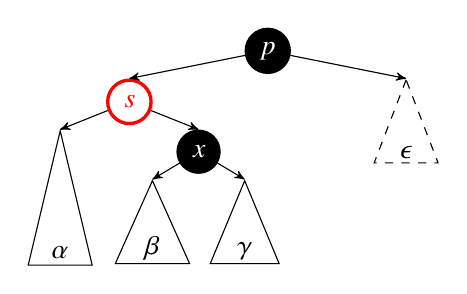
\begin{tikzpicture}[->,>=stealth',level/.style={sibling distance = 10em/#1, level distance = 1em}, child anchor=north]
\node [node_b] {$p$}
child {
	node [node_r] {$s$}
	child {
		node [node_tree_high1] {$\alpha$}
	}
	child {
		node [node_b] {$x$}
		child {
			node [node_tree] {$\beta$}
		}
		child {
			node [node_tree] {$\gamma$}
		}
	}
}
child {
	node [node_tree_low] {$\epsilon$}
}
;
\end{tikzpicture}
\end{center}

\subsubsection{Transformation}


\begin{enumerate}
\item The nodes $p$ and $s$ create a 3-node with a single subtree which has a
too low black height. This can be fixed by converting it in a 2-node and melding
two subtrees together to form one tree with the right black height.

The first step is to rotate $p$ to the right. This converts the left leaning
3-node under $p$ to a right leaning 3-node under $s$.

\begin{center}
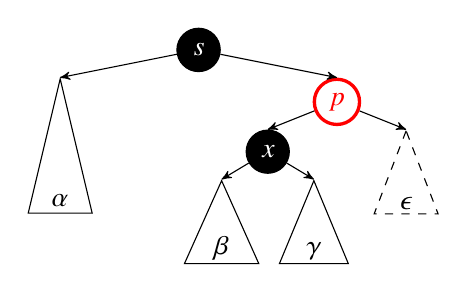
\begin{tikzpicture}[->,>=stealth',level/.style={sibling distance = 10em/#1, level distance = 1em}, child anchor=north]
\node [node_b] {$s$}
child {
	node [node_tree_high1] {$\alpha$}
}
child {
	node [node_r] {$p$}
	child {
		node [node_b] {$x$}
		child {
			node [node_tree] {$\beta$}
		}
		child {
			node [node_tree] {$\gamma$}
		}
	}
	child {
		node [node_tree_low] {$\epsilon$}
	}
}
;
\end{tikzpicture}
\end{center}


\item Switching the colors of $p$ and $x$ creates a new 3-node. All of the
subtrees of this 3-node have the same black height. The rebalance process is
finished after that.

\begin{center}
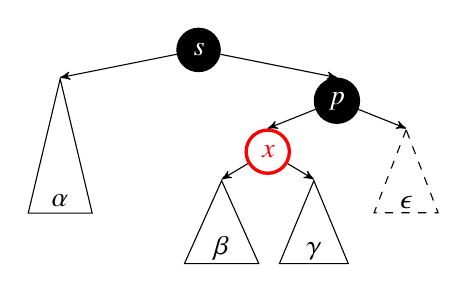
\begin{tikzpicture}[->,>=stealth',level/.style={sibling distance = 10em/#1, level distance = 1em}, child anchor=north]
\node [node_b] {$s$}
child {
	node [node_tree_high1] {$\alpha$}
}
child {
	node [node_b] {$p$}
	child {
		node [node_r] {$x$}
		child {
			node [node_tree] {$\beta$}
		}
		child {
			node [node_tree] {$\gamma$}
		}
	}
	child {
		node [node_tree_low] {$\epsilon$}
	}
}
;
\end{tikzpicture}
\end{center}


\end{enumerate}

%%%%%%%%%%%%%%%%%%%%%%%%%%%%%%%%%%%%%%%%%%%%%%%%%%%%%%%%%%%%%%%%%%%%%%%%%%%%%%%%
% rb_erase_right_adjust_red
%%%%%%%%%%%%%%%%%%%%%%%%%%%%%%%%%%%%%%%%%%%%%%%%%%%%%%%%%%%%%%%%%%%%%%%%%%%%%%%%
\newpage
\subsection{Low Right Subtree, Restructure with Adjust and Recolor}

\subsubsection{Prerequisites}

\begin{center}
\begin{tabular}{|r||l|l|}
\hline
node		&	black height	&	comment	\\
\hline
\hline
$p$		&	imbalanced	&	is black	\\\hline
$s$		&	$h+1$	&	red sibling of $\epsilon$ root	\\\hline
$x$		&	$h+1$	&	black left child of $s$	\\\hline
$y$		&	$h$	&	red left child of $x$	\\\hline
$\epsilon$	&	$h$	&	black node was removed from subtree, right child of $p$	\\\hline
$\alpha$	&	$h+1$	&		\\\hline
$\beta$		&	$h$	&		\\\hline
$\gamma$	&	$h$	&		\\\hline
$\delta$	&	$h$	&		\\\hline
\end{tabular}
\end{center}

\begin{center}
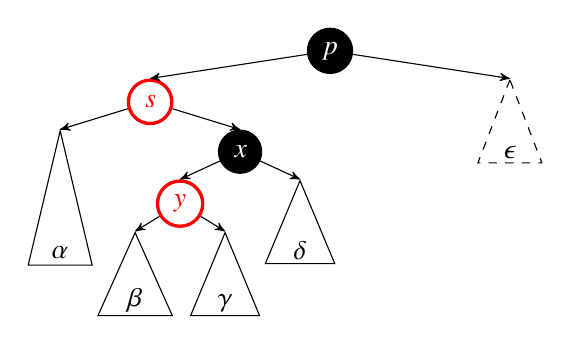
\begin{tikzpicture}[->,>=stealth',level/.style={sibling distance = 13em/#1, level distance = 1em}, child anchor=north]
\node [node_b] {$p$}
child {
	node [node_r] {$s$}
	child {
		node [node_tree_high1] {$\alpha$}
	}
	child {
		node [node_b] {$x$}
		child {
			node [node_r] {$y$}
			child {
				node [node_tree] {$\beta$}
			}
			child {
				node [node_tree] {$\gamma$}
			}
		}
		child {
			node [node_tree] {$\delta$}
		}
	}
}
child {
	node [node_tree_low] {$\epsilon$}
}
;
\end{tikzpicture}
\end{center}

\subsubsection{Transformation}

\begin{enumerate}
\item The black node from the left subtree has to be transferred to the right
to increase its height. But at first the left subtree has to be prepared
to avoid a reduction of its black height. This is done by rotating $s$ to the
left. This breaks the balance of the subtress under $s$.

\begin{center}
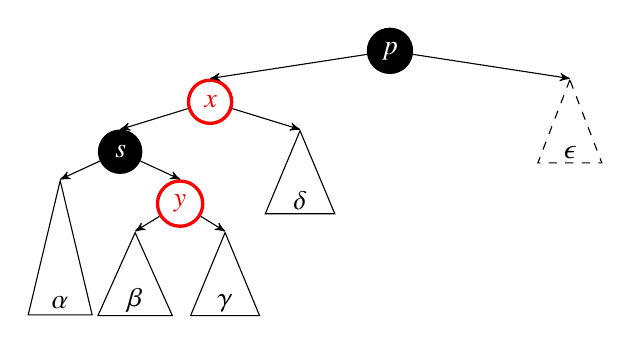
\begin{tikzpicture}[->,>=stealth',level/.style={sibling distance = 13em/#1, level distance = 1em}, child anchor=north]
\node [node_b] {$p$}
child {
	node [node_r] {$x$}
	child {
		node [node_b] {$s$}
		child {
			node [node_tree_high1] {$\alpha$}
		}
		child {
			node [node_r] {$y$}
			child {
				node [node_tree] {$\beta$}
			}
			child {
				node [node_tree] {$\gamma$}
			}
		}
	}
	child {
		node [node_tree] {$\delta$}
	}
}
child {
	node [node_tree_low] {$\epsilon$}
}
;
\end{tikzpicture}
\end{center}


\item The imbalance under $s$ is solved by switching the colors of $s$ and $x$.
This creates two consecutive left red nodes.

\begin{center}
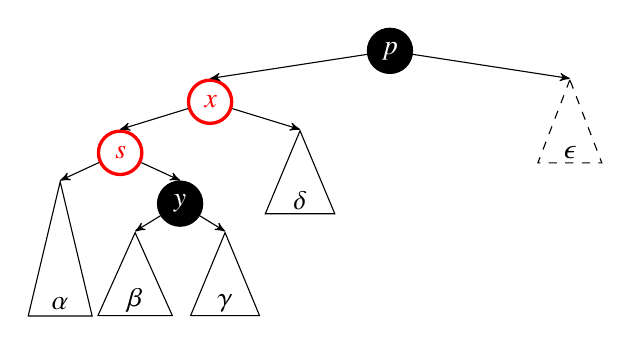
\begin{tikzpicture}[->,>=stealth',level/.style={sibling distance = 13em/#1, level distance = 1em}, child anchor=north]
\node [node_b] {$p$}
child {
	node [node_r] {$x$}
	child {
		node [node_r] {$s$}
		child {
			node [node_tree_high1] {$\alpha$}
		}
		child {
			node [node_b] {$y$}
			child {
				node [node_tree] {$\beta$}
			}
			child {
				node [node_tree] {$\gamma$}
			}
		}
	}
	child {
		node [node_tree] {$\delta$}
	}
}
child {
	node [node_tree_low] {$\epsilon$}
}
;
\end{tikzpicture}
\end{center}


\item The transfer or the node to the right is done by rotating $p$ to the right.
This automatically solves the two consecutive red nodes in the left tree while
preserving the black height.

\begin{center}
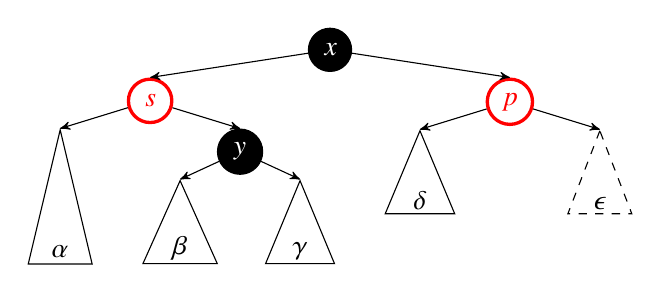
\begin{tikzpicture}[->,>=stealth',level/.style={sibling distance = 13em/#1, level distance = 1em}, child anchor=north]
\node [node_b] {$x$}
child {
	node [node_r] {$s$}
	child {
		node [node_tree_high1] {$\alpha$}
	}
	child {
		node [node_b] {$y$}
		child {
			node [node_tree] {$\beta$}
		}
		child {
			node [node_tree] {$\gamma$}
		}
	}
}
child {
	node [node_r] {$p$}
	child {
		node [node_tree] {$\delta$}
	}
	child {
		node [node_tree_low] {$\epsilon$}
	}
}
;
\end{tikzpicture}
\end{center}


\item The black height in the right subtree is still too low but the subtree
has a red node as its root. This 4-node is not allowed in a 2-3 red-black tree
but can be used to fix the imbalance. $p$ is recolored to black to increase the
black height of the right subtree. The rebalance process is finished after that.

\begin{center}
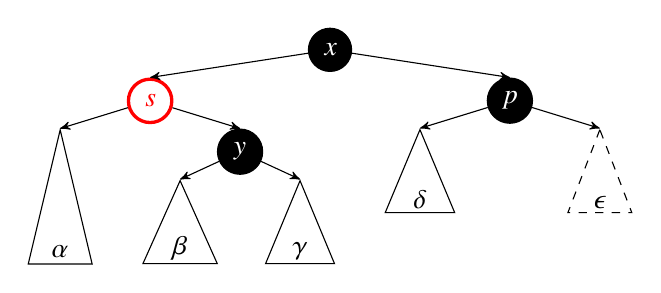
\begin{tikzpicture}[->,>=stealth',level/.style={sibling distance = 13em/#1, level distance = 1em}, child anchor=north]
\node [node_b] {$x$}
child {
	node [node_r] {$s$}
	child {
		node [node_tree_high1] {$\alpha$}
	}
	child {
		node [node_b] {$y$}
		child {
			node [node_tree] {$\beta$}
		}
		child {
			node [node_tree] {$\gamma$}
		}
	}
}
child {
	node [node_b] {$p$}
	child {
		node [node_tree] {$\delta$}
	}
	child {
		node [node_tree_low] {$\epsilon$}
	}
}
;
\end{tikzpicture}
\end{center}

\end{enumerate}


%%%%%%%%%%%%%%%%%%%%%%%%%%%%%%%%%%%%%%%%%%%%%%%%%%%%%%%%%%%%%%%%%%%%%%%%%%%%%%%%
% rb_erase_right_restructure
%%%%%%%%%%%%%%%%%%%%%%%%%%%%%%%%%%%%%%%%%%%%%%%%%%%%%%%%%%%%%%%%%%%%%%%%%%%%%%%%
\newpage
\subsection{Low Right Subtree, Restructure with Recolor}

\subsubsection{Prerequisites}

\begin{center}
\begin{tabular}{|r||l|l|}
\hline
node		&	black height	&	comment	\\
\hline
\hline
$p$		&	imbalanced	&		\\\hline
$s$		&	$h+1$	&	black sibling of $\epsilon$ root	\\\hline
$x$		&	$h$	&	red left child of $s$	\\\hline
$\epsilon$	&	$h$	&	black node was removed from subtree, right child of $p$	\\\hline
$\alpha$	&	$h$	&		\\\hline
$\beta$		&	$h$	&		\\\hline
$\gamma$	&	$h$	&		\\\hline
\end{tabular}
\end{center}

\begin{center}
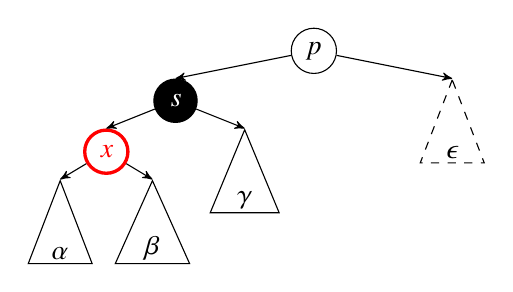
\begin{tikzpicture}[->,>=stealth',level/.style={sibling distance = 10em/#1, level distance = 1em}, child anchor=north]
\node [node_rb] {$p$}
child {
	node [node_b] {$s$}
	child {
		node [node_r] {$x$}
		child {
			node [node_tree] {$\alpha$}
		}
		child {
			node [node_tree] {$\beta$}
		}
	}
	child {
		node [node_tree] {$\gamma$}
	}
}
child {
	node [node_tree_low] {$\epsilon$}
}
;
\end{tikzpicture}
\end{center}

\subsubsection{Transformation}

\begin{enumerate}
\item $p$ can be rotated to the right to fix the black height in the
right subtree.

\begin{center}
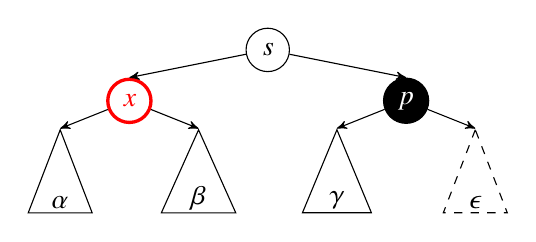
\begin{tikzpicture}[->,>=stealth',level/.style={sibling distance = 10em/#1, level distance = 1em}, child anchor=north]
\node [node_rb] {$s$}
child {
	node [node_r] {$x$}
	child {
		node [node_tree] {$\alpha$}
	}
	child {
		node [node_tree] {$\beta$}
	}
}
child {
	node [node_b] {$p$}
	child {
		node [node_tree] {$\gamma$}
	}
	child {
		node [node_tree_low] {$\epsilon$}
	}
}
;
\end{tikzpicture}
\end{center}


\item The left subtree now has a too low black height compared to the right
tree. But the red $x$ can simply be recolored to black to increase the black
height again and to fix the misbalance in the tree. The rebalance process is
finished after that.

\begin{center}
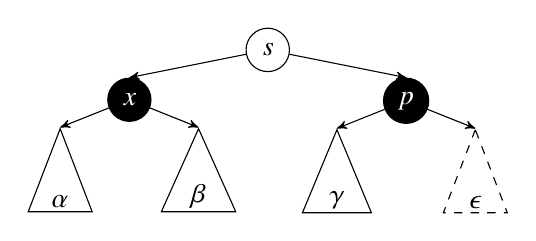
\begin{tikzpicture}[->,>=stealth',level/.style={sibling distance = 10em/#1, level distance = 1em}, child anchor=north]
\node [node_rb] {$s$}
child {
	node [node_b] {$x$}
	child {
		node [node_tree] {$\alpha$}
	}
	child {
		node [node_tree] {$\beta$}
	}
}
child {
	node [node_b] {$p$}
	child {
		node [node_tree] {$\gamma$}
	}
	child {
		node [node_tree_low] {$\epsilon$}
	}
}
;
\end{tikzpicture}
\end{center}


\end{enumerate}


%%%%%%%%%%%%%%%%%%%%%%%%%%%%%%%%%%%%%%%%%%%%%%%%%%%%%%%%%%%%%%%%%%%%%%%%%%%%%%%%
% rb_erase_right_recolor_red
%%%%%%%%%%%%%%%%%%%%%%%%%%%%%%%%%%%%%%%%%%%%%%%%%%%%%%%%%%%%%%%%%%%%%%%%%%%%%%%%
\newpage
\subsection{Low Right Subtree, Recolor under red parent}

\subsubsection{Prerequisites}

\begin{center}
\begin{tabular}{|r||l|l|}
\hline
node		&	black height	&	comment	\\
\hline
\hline
$p$		&	imbalanced	&	is red	\\\hline
$s$		&	$h+1$	&	black sibling of $\epsilon$ root	\\\hline
$\epsilon$	&	$h$	&	black node was removed from subtree, right child of $p$	\\\hline
$\alpha$	&	$h$	&		\\\hline
$\beta$		&	$h$	&		\\\hline
\end{tabular}
\end{center}

\begin{center}
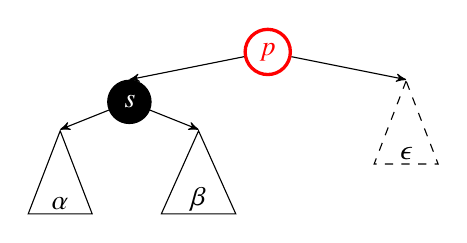
\begin{tikzpicture}[->,>=stealth',level/.style={sibling distance = 10em/#1, level distance = 1em}, child anchor=north]
\node [node_r] {$p$}
child {
	node [node_b] {$s$}
	child {
		node [node_tree] {$\alpha$}
	}
	child {
		node [node_tree] {$\beta$}
	}
}
child {
	node [node_tree_low] {$\epsilon$}
}
;
\end{tikzpicture}
\end{center}

\subsubsection{Transformation}

\begin{enumerate}

\item Switching the colors of $p$ und $s$ fixes the black heights. The black
height of the left subtree is decreased (and therefore equal to the right
subtree) while the black height under $p$ is increased. The imbalance is
solved.

\begin{center}
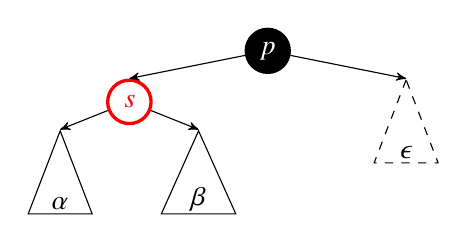
\begin{tikzpicture}[->,>=stealth',level/.style={sibling distance = 10em/#1, level distance = 1em}, child anchor=north]
\node [node_b] {$p$}
child {
	node [node_r] {$s$}
	child {
		node [node_tree] {$\alpha$}
	}
	child {
		node [node_tree] {$\beta$}
	}
}
child {
	node [node_tree_low] {$\epsilon$}
}
;
\end{tikzpicture}
\end{center}


\end{enumerate}


%%%%%%%%%%%%%%%%%%%%%%%%%%%%%%%%%%%%%%%%%%%%%%%%%%%%%%%%%%%%%%%%%%%%%%%%%%%%%%%%
% rb_erase_right_recolor_black
%%%%%%%%%%%%%%%%%%%%%%%%%%%%%%%%%%%%%%%%%%%%%%%%%%%%%%%%%%%%%%%%%%%%%%%%%%%%%%%%
\newpage
\subsection{Low Right Subtree, Recolor under black parent}

\subsubsection{Prerequisites}

\begin{center}
\begin{tabular}{|r||l|l|}
\hline
node		&	black height	&	comment	\\
\hline
\hline
$p$		&	imbalanced	&	is black	\\\hline
$s$		&	$h+1$	&	black sibling of $\epsilon$ root	\\\hline
$\epsilon$	&	$h$	&	black node was removed from subtree, right child of $p$	\\\hline
$\alpha$	&	$h$	&	root of $\alpha$ must be black or NULL	\\\hline
$\beta$		&	$h$	&		\\\hline
\end{tabular}
\end{center}

\begin{center}
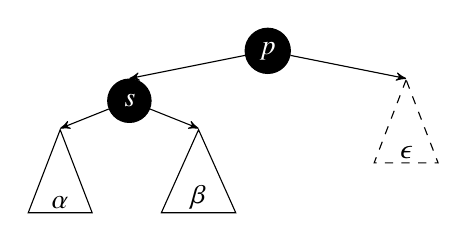
\begin{tikzpicture}[->,>=stealth',level/.style={sibling distance = 10em/#1, level distance = 1em}, child anchor=north]
\node [node_b] {$p$}
child {
	node [node_b] {$s$}
	child {
		node [node_tree] {$\alpha$}
	}
	child {
		node [node_tree] {$\beta$}
	}
}
child {
	node [node_tree_low] {$\epsilon$}
}
;
\end{tikzpicture}
\end{center}

\subsubsection{Transformation}

\begin{enumerate}
\item The imbalance cannot be solved using local operations. Instead the black
height of the right subtree has to be decreased to have the same height as
the left subtree. This is done by recoloring $s$.

\begin{center}
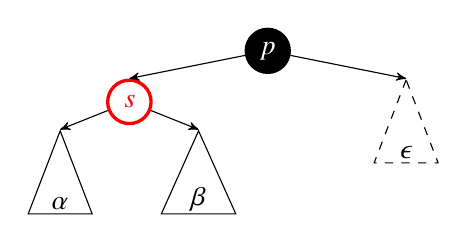
\begin{tikzpicture}[->,>=stealth',level/.style={sibling distance = 10em/#1, level distance = 1em}, child anchor=north]
\node [node_b] {$p$}
child {
	node [node_r] {$s$}
	child {
		node [node_tree] {$\alpha$}
	}
	child {
		node [node_tree] {$\beta$}
	}
}
child {
	node [node_tree_low] {$\epsilon$}
}
;
\end{tikzpicture}
\end{center}


\item The subtree under $s$ has its black height reduced by 1. This problem
has to be propagated further upward the tree to get it solved.


\end{enumerate}


%%%%%%%%%%%%%%%%%%%%%%%%%%%%%%%%%%%%%%%%%%%%%%%%%%%%%%%%%%%%%%%%%%%%%%%%%%%%%%%%
% rb_delete_color root node is red
%%%%%%%%%%%%%%%%%%%%%%%%%%%%%%%%%%%%%%%%%%%%%%%%%%%%%%%%%%%%%%%%%%%%%%%%%%%%%%%%
\newpage
\subsection{Root is red}

\subsubsection{Prerequisites}

\begin{center}
\begin{tabular}{|r||l|l|}
\hline
node		&	black height	&	comment	\\
\hline
\hline
$n$		&	$h$	&	is red and the root of the tree	\\\hline
$\alpha$	&	$h$	&		\\\hline
$\beta$		&	$h$	&		\\\hline
\end{tabular}
\end{center}

A root of a tree always has to be black.

\begin{center}
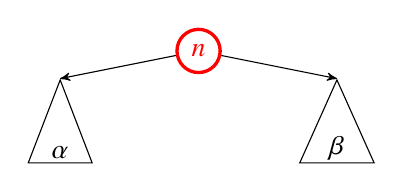
\begin{tikzpicture}[->,>=stealth',level/.style={sibling distance = 10em/#1, level distance = 1em}, child anchor=north]
\node [node_r] {$n$}
child {
	node [node_tree] {$\alpha$}
}
child {
	node [node_tree] {$\beta$}
}
;
\end{tikzpicture}
\end{center}

\subsubsection{Transformation}

\begin{enumerate}
\item Changing the color of $n$ increases the black height of the tree. But
no imbalance can be introduced because $\alpha$ and $\beta$ are already balanced
and $n$ has no parent which could get unbalanced.

\begin{center}
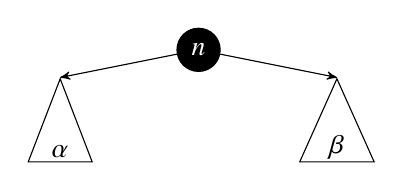
\begin{tikzpicture}[->,>=stealth',level/.style={sibling distance = 10em/#1, level distance = 1em}, child anchor=north]
\node [node_b] {$n$}
child {
	node [node_tree] {$\alpha$}
}
child {
	node [node_tree] {$\beta$}
}
;
\end{tikzpicture}
\end{center}


\item Rebalance can always always stop after $n$ is marked as black.

\end{enumerate}

\end{document}
